%!TEX root = ../thesis.tex

\section{Local Deployment}
\label{sec:local_infrastructure}

The local deployments consists of the residential communication gateway and the deployed thermostats with their wireless adapters. The communication gateway collects the data read from the thermostats and sends it to a remote web server. The thermostats are programmable and allow us to modify their behaviour by replacing and adapting the flashed firmware. This project uses the work of previous lab projects as a basis to build upon. The primary focus is to improve the basic functionality of the communication gateway and create an unified but loosely coupled infrastructure by using the RESTful API provided by the server.
See also Figure~\ref{fig:residence_layout} for an overview of the local deployment.

\begin{figure}[h]
\begin{center}
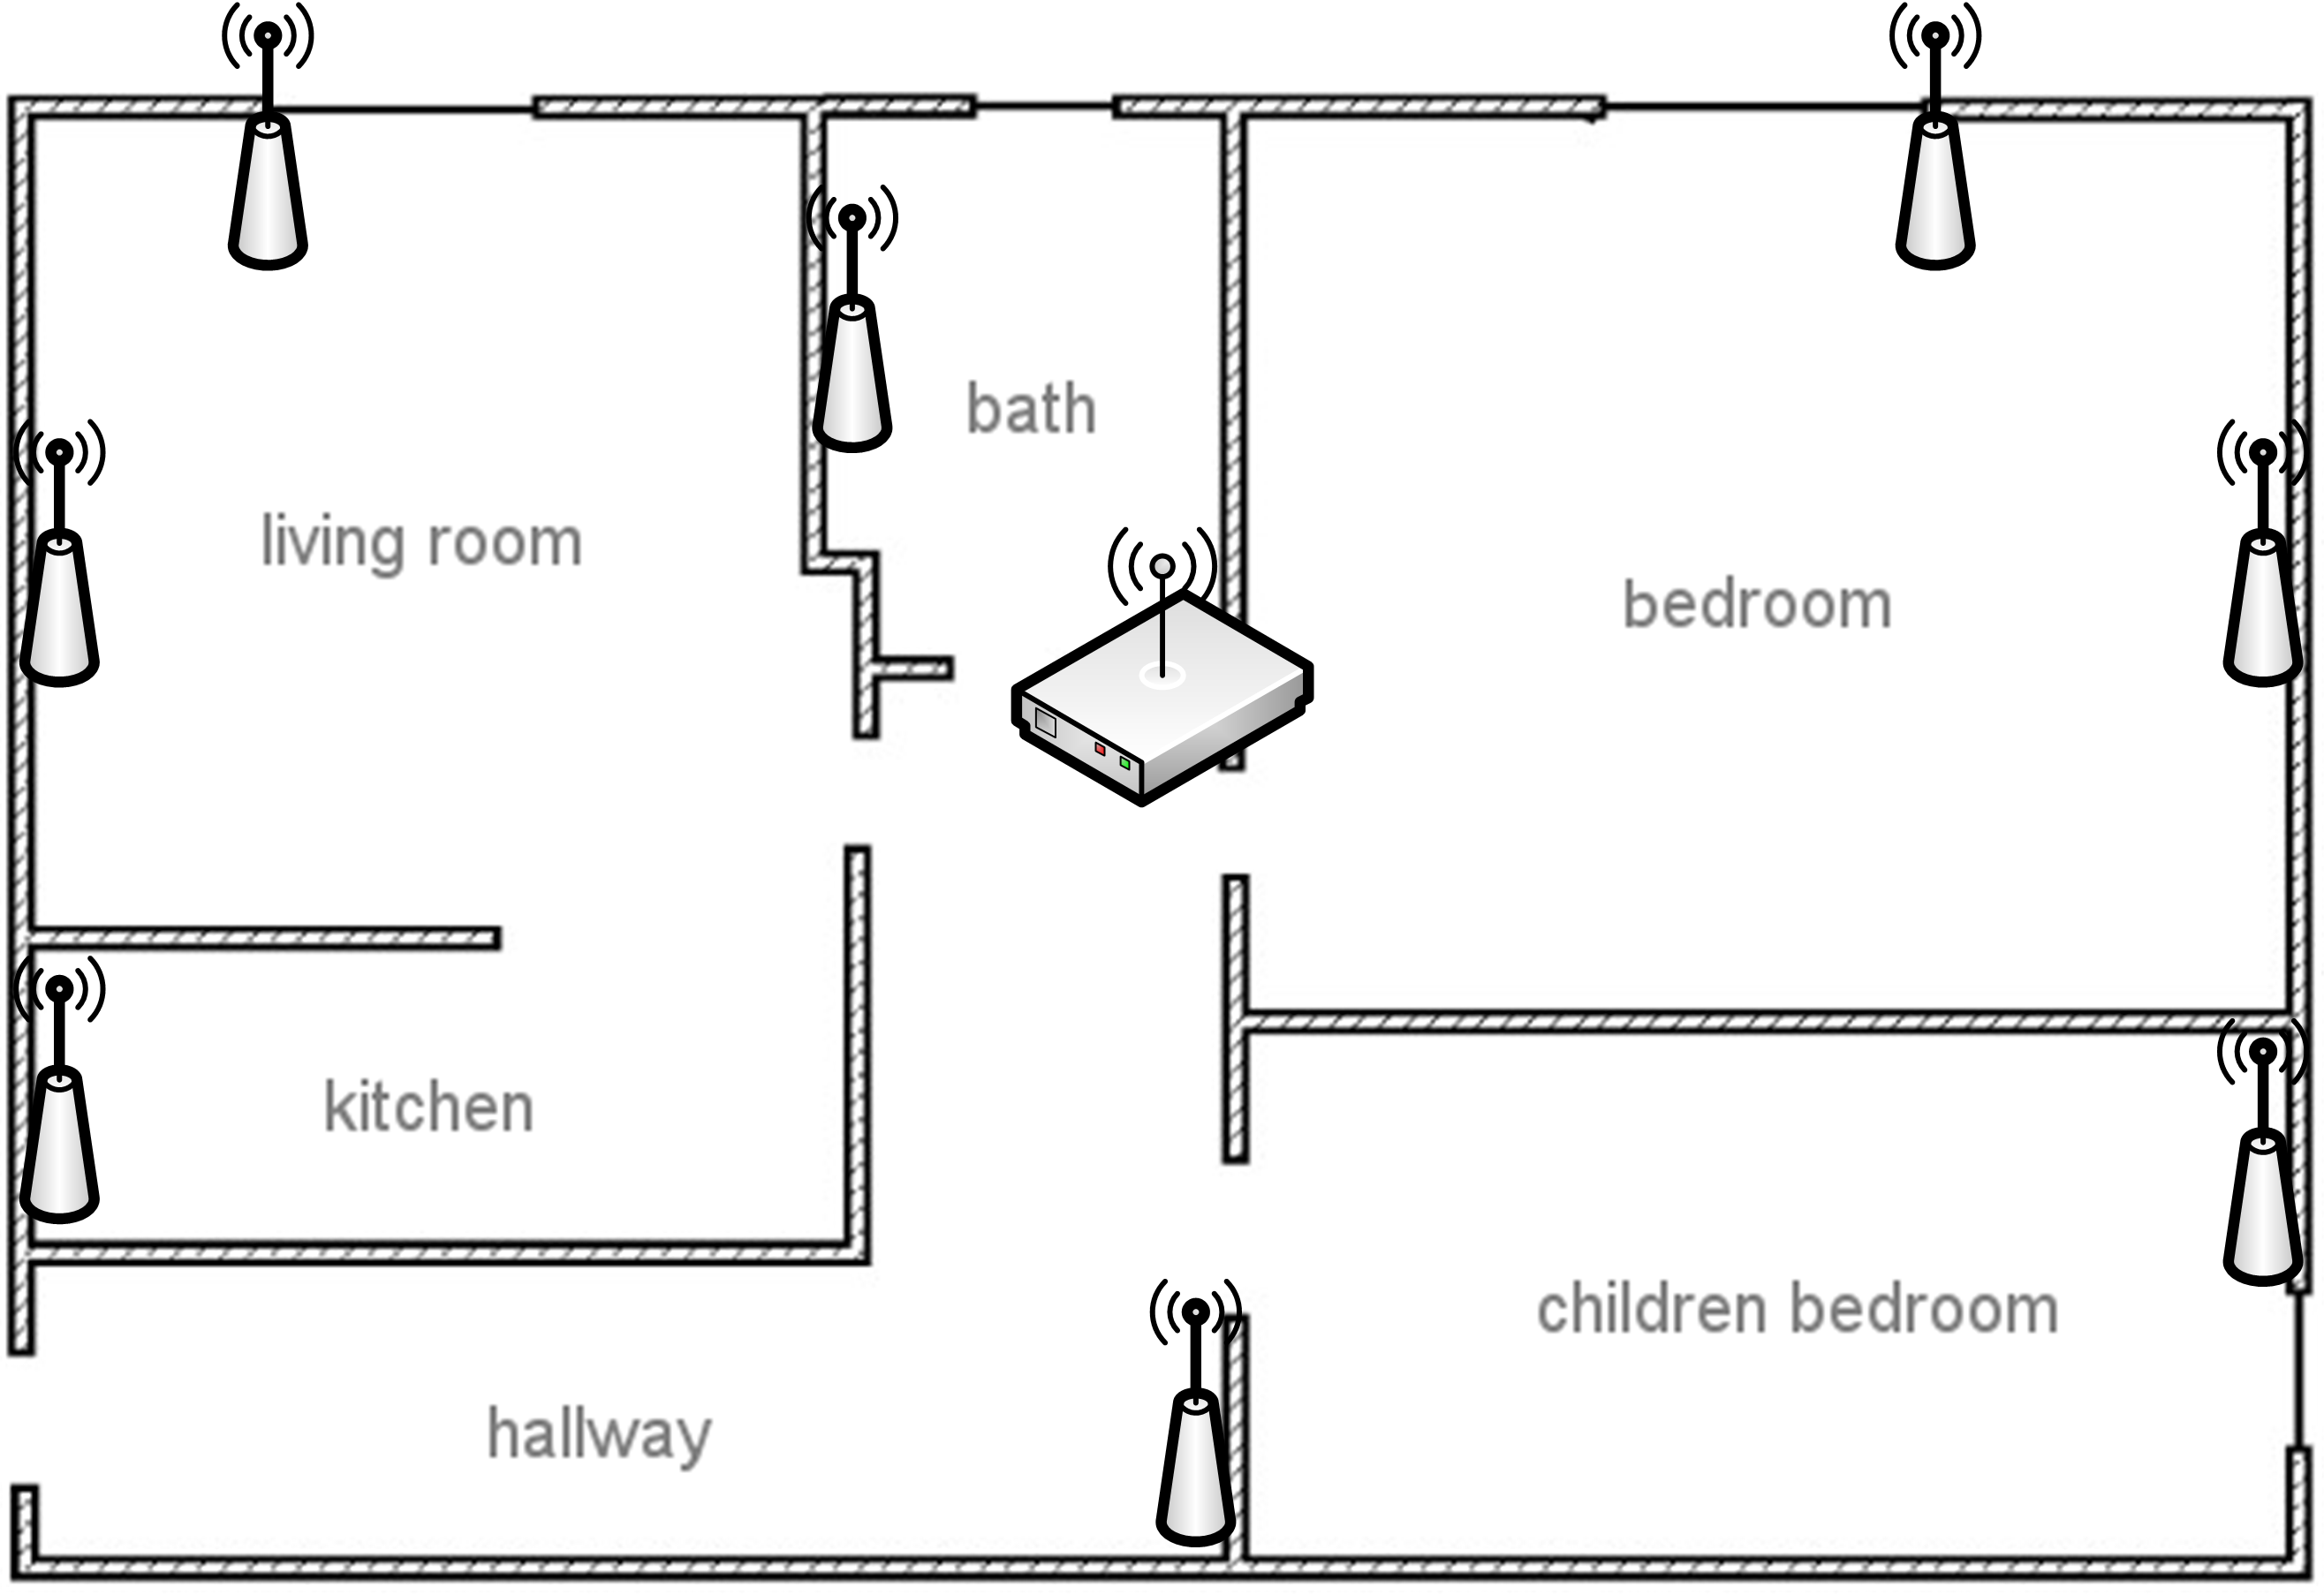
\includegraphics[width=0.8\textwidth]{images/residence_layout_schema.png}
\end{center}
\caption{Example of a residence layout depicting a possible deployment. The local communication gateway is installed in the hallway, connected to the internet and has wireless connections to the deployed thermostats represented as antennas. Source of the original image: \url{http://www.haus-topplicht.de/wp-content/uploads/2013/12/planwohnung2.jpg}}
\label{fig:residence_layout}
\end{figure}

\subsection{Existing Infrastructure}

This lab project builds upon work previously done at the Distributed System Group\footnote{\url{https://www.vs.inf.ethz.ch/}}. 

\subsubsection*{Hardware}

Thermostats, etc

\subsubsection*{Software}

Willis Scripts

\subsection{Design Goals}

Simple, Reliable, Failure resistant

\subsection{Platform and Frameworks}

tunslip6, Python, COAP, aiocoap, requests

\subsection{Implementation}

The communication gateway collects, caches and processes the data read from the thermostats as also the control commands from the server. The local communication gateway works as a proxy server and enables the local deployment to operate independently from the connection to the remote server. This way the last downloaded heating schedule is kept and operated until the server connection is be reestablished. 
%Die grundlegende Einheit jedes Deployments ist die Residence. Eine Residence entspricht genau einem installiertem lokalen System, das die gelesenen Daten der Thermostate sowie Steuerbefehle des Servers sammelt, cached and ausführt. Das lokale Gerät arbeitet als ein lokales Gateway und sorgt dafür, dass der lokale Teil unabhängig von der Verbindung mit dem remote Server funktioniert.
% Temperaturen und andere Meta-Daten von den angebundenen Thermostaten sammelt und cached.

